% vim: set ts=4 sw=4 tw=80 noexpandtab:

\documentclass{42-en}

%******************************************************************************%
%                                                                              %
%                                   Prologue                                   %
%                                                                              %
%******************************************************************************%
\usepackage[
    type={CC},
    modifier={by-nc-sa},
    version={4.0},
]{doclicense}
\usepackage{amsmath} % The amsmath package provides commands to typeset matrices with different delimiters. 
\usepackage{epigraph}
\usepackage[parfill]{parskip}
\setlength\epigraphwidth{.95\textwidth}
%****************************************************************%
%                  Re/definition of commands                     %
%****************************************************************%

\newcommand{\ailogo}[1]{\def \@ailogo {#1}}\ailogo{assets/42ai_logo.pdf}

%%  Redefine \maketitle
\makeatletter
\def \maketitle {
  \begin{titlepage}
    \begin{center}
	%\begin{figure}[t]
	  %\includegraphics[height=8cm]{\@ailogo}
	  
\includegraphics[height=8cm]{assets/42ai_logo.pdf}
	%\end{figure}
      \vskip 5em
      {\huge \@title}
      \vskip 2em
      {\LARGE \@subtitle}
      \vskip 4em
    \end{center}
    %\begin{center}
	  %\@author
    %\end{center}
	%\vskip 5em
  \vfill
  \begin{center}
    \emph{\summarytitle : \@summary}
  \end{center}
  \vspace{2cm}
  %\vskip 5em
  %\doclicenseThis
  \end{titlepage}
}
\makeatother

\makeatletter
\def \makeheaderfilesforbidden
{
  \noindent
  \begin{tabularx}{\textwidth}{|X X  X X|}
    \hline
  \multicolumn{1}{|>{\raggedright}m{1cm}|}
  {\vskip 2mm 
\includegraphics[height=1cm]{assets/42ai_logo.pdf}} &
  \multicolumn{2}{>{\centering}m{12cm}}{\small Exercise : \@exnumber } &
  \multicolumn{1}{ >{\raggedleft}p{1.5cm}|}
%%              {\scriptsize points : \@exscore} \\ \hline
              {} \\ \hline

  \multicolumn{4}{|>{\centering}m{15cm}|}
              {\small \@extitle} \\ \hline

  \multicolumn{4}{|>{\raggedright}m{15cm}|}
              {\small Turn-in directory : \ttfamily
                $ex\@exnumber/$ }
              \\ \hline
  \multicolumn{4}{|>{\raggedright}m{15cm}|}
              {\small Files to turn in : \ttfamily \@exfiles }
              \\ \hline

  \multicolumn{4}{|>{\raggedright}m{15cm}|}
              {\small Forbidden functions : \ttfamily \@exforbidden }
              \\ \hline

%%  \multicolumn{4}{|>{\raggedright}m{15cm}|}
%%              {\small Remarks : \ttfamily \@exnotes }
%%              \\ \hline
\end{tabularx}
%% \exnotes
\exrules
\exmake
\exauthorize{None}
\exforbidden{None}
\extitle{}
\exnumber{}
}
\makeatother

%%  Syntactic highlights
\makeatletter
\newenvironment{pythoncode}{%
  \VerbatimEnvironment
  \usemintedstyle{emacs}
  \minted@resetoptions
  \setkeys{minted@opt}{bgcolor=black,formatcom=\color{lightgrey},fontsize=\scriptsize}
  \begin{figure}[ht!]
    \centering
    \begin{minipage}{16cm}
      \begin{VerbatimOut}{\jobname.pyg}}
{%[
      \end{VerbatimOut}
      \minted@pygmentize{c}
      \DeleteFile{\jobname.pyg}
    \end{minipage}
\end{figure}}
\makeatother

\usemintedstyle{native}

\begin{document}

% =============================================================================%
%                     =====================================                    %

\title{Machine Learning - Module 00}
\subtitle{Stepping into Machine Learning}
\author{
  Maxime Choulika (cmaxime), Pierre Peigné (ppeigne), Matthieu David (mdavid)
}

\summary
{
  You will start by reviewing some linear algebra and statistics.
  Then you will implement your first model and learn how to evaluate its performances.
}

\maketitle
%******************************************************************************%
%                                                                              %
%                        Section usefull ressources                            %
%                          for ML Modules                                      %
%                                                                              %
%******************************************************************************%


\chapter*{Notions and ressources}

\section*{Notions of the module}
Regularization, overfitting. Regularized loss function, regularized gradient descent.  
Regularized linear regression. Regularized logistic regression.

\section*{Useful Ressources}

You are strongly advise to use the following resource:
\href{https://www.coursera.org/learn/machine-learning}{Machine Learning MOOC - Stanford}
These videos are available at no cost; simply log in, select "Enroll for Free", and choose "audit the course for free" in the popup window.
The following sections of the course are pertinent to today's exercises:

\newpage

\subsection*{Week 3: Classification}

\subsubsection*{Classification with logistic regression (already seen on module 03)}
\begin{itemize}
  \item Motivations
  \item Logistic regression
  \item Decision boundary
\end{itemize}

\subsubsection*{Cost function for logistic regression (already seen on module 03)}
\begin{itemize}
  \item Cost function for logistic regression
  \item Simplified Cost Function for Logistic Regression
\end{itemize}

\subsubsection*{Gradient descent for logistic regression (already seen on module 03)}
\begin{itemize}
  \item Gradient Descent Implementation
\end{itemize}

\subsubsection*{The problem of overfitting (New !!!)}
\begin{itemize}
  \item The problem of overfitting
  \item Addressing overfitting
  \item Cost function with regularization
  \item Regularized linear regression
  \item Regularized logistic regression  
\end{itemize}


\emph{All videos above are available also on this \href{https://youtube.com/playlist?list=PLkDaE6sCZn6FNC6YRfRQc_FbeQrF8BwGI&feature=shared}{Andrew Ng's YouTube playlist}, videos from 31 to 36 (already seen on module 03) and 37 to 41 (new !!!).}
%******************************************************************************%
%                                                                              %
%                        Common Instructions                                   %
%                          for Python Projects                                 %
%                                                                              %
%******************************************************************************%

\chapter*{Common Instructions}
\begin{itemize}
  \item The version of Python recommended to use is 3.7, you can
  check the version of Python with the following command: \texttt{python -V}
  
  \item The norm: during this piscine, it is recommended to follow the
  \href{https://www.python.org/dev/peps/pep-0008/}{PEP 8 standards}, though it is not mandatory.
  You can install \href{https://pypi.org/project/pycodestyle}{pycodestyle} which
  is a tool to check your Python code.
  
  \item The function \texttt{eval} is never allowed.
  
  \item The exercises are ordered from the easiest to the hardest.
  
  \item Your exercises are going to be evaluated by someone else,
  so make sure that your variable names and function names are appropriate and civil. 
  
  \item Your manual is the internet.
  
  \item You can also ask questions on the {https://discord.gg/8Vvb6QMCZq}{42AI} discord.
  
  \item If you find any issue or mistakes in the subject please create an issue on \href{https://github.com/42-AI/bootcamp_python/issues}{42AI repository on Github}.  
  
  \item We encourage you to create test programs for your
  project even though this work \textbf{won't have to be
  submitted and won't be graded}. It will give you a chance
  to easily test your work and your peers’ work. You will find
  those tests especially useful during your defence. Indeed,
  during defence, you are free to use your tests and/or the
  tests of the peer you are evaluating.
  
  \item Submit your work to your assigned git repository. Only the work in the
  git repository will be graded. If Deepthought is assigned to grade your
  work, it will be run after your peer-evaluations.
  If an error happens in any section of your work during Deepthought's grading,
  the evaluation will stop.
\end{itemize}

\newpage
\tableofcontents
\startexercices

%                     =====================================                    %
% =============================================================================%


%******************************************************************************%
%                                                                              %
%                                   Exercises                                  %
%                                                                              %
%******************************************************************************%

% ============================================== %
% ===========================(start ex 00)       %
\chapter{Exercise 00}
\extitle{The Matrix}
\turnindir{ex00}
\exnumber{00}
\exfiles{matrix.py, test.py}
\exforbidden{Numpy}
\makeheaderfilesforbidden

% ================================== %
\section*{Objective}
% ---------------------------------- %
Manipulation and understanding of basic matrix operations.\\
In this exercise, you have to create a \texttt{Matrix} and a \texttt{Vector} class.
The goal is to have matrices and be able to perform both matrix-matrix operation
and matrix-vector operations with them.

% ================================== %
\section*{Instructions}
% ---------------------------------- %
You will provide a testing file to prove that your classes works as expected.\\

Your \texttt{Matrix} class must have the following 2 attributes: 
\begin{itemize}
  \item \texttt{data}: list of lists
  \item \texttt{shape}: the dimensions of the matrix as a tuple (rows, columns)
\end{itemize}

You should be able to initialize the object with either:
\begin{itemize}
  \item the elements of the matrix as a list of lists: \texttt{Matrix([[1.0, 2.0], [3.0, 4.0]])}
  \item a shape: \texttt{Matrix((3, 3))} (the matrix will be filled with zeros by default)
\end{itemize}

You will implement all the following built-in functions (called \texttt{magic/special methods}) for your \texttt{Matrix} class:

\begin{minted}[bgcolor=darcula-back,formatcom=\color{lightgrey},fontsize=\scriptsize]{python}
    # add : only matrices of same dimensions.
    __add__
    __radd__
    # sub : only matrices of same dimensions.
    __sub__
    __rsub__
    # div : only scalars.
    __truediv__
    __rtruediv__
    # mul : scalars, vectors and matrices , can have errors with vectors and matrices, 
    # returns a Vector if we perform Matrix * Vector mutliplication.
    __mul__
    __rmul__
    __str__
    __repr__
\end{minted}

You will also implement: 
\begin{itemize}
  \item a \texttt{.T()} method which returns the transpose of the matrix (see examples below),
\end{itemize}


Then, you must create a \texttt{Vector} class that inherit from Matrix.
At initialization, you must check that a column or a row vector is passed as the data argument.
If not, you must send an error message :

\begin{minted}[bgcolor=darcula-back,formatcom=\color{lightgrey},fontsize=\scriptsize]{python}
  v1 = Vector([[1, 2, 3]]) # create a row vector
  v2 = Vector([[1], [2], [3]]) # create a column vector
  v3 = Vector([[1, 2], [3, 4]]) # return an error
\end{minted}

\par
For \texttt{Vector}, you must implement:
\begin{itemize}
  \item a \texttt{.dot(self, v: Vector)} method which returns the dot product between the current vector and v. If shapes don't match, you must properly display errors.
\end{itemize}

\warn{
  Caution: when you do operations between Vector, it must return a Vector and not a Matrix 
}
\hint{
  type(self)
}

\section*{Examples}

\begin{minted}[bgcolor=darcula-back,formatcom=\color{lightgrey},fontsize=\scriptsize]{python}
m1 = Matrix([[0.0, 1.0], [2.0, 3.0], [4.0, 5.0]])
m1.shape
# Output:
(3, 2)

m1.T()
# Output:
Matrix([[0., 2., 4.], [1., 3., 5.]])

m1.T().shape
# Output:
(2, 3)
\end{minted}
\begin{minted}[bgcolor=darcula-back,formatcom=\color{lightgrey},fontsize=\scriptsize]{python}
m1 = Matrix([[0., 2., 4.], [1., 3., 5.]])
m1.shape
# Output:
(2, 3)

m1.T()
# Output:
Matrix([[0.0, 1.0], [2.0, 3.0], [4.0, 5.0]])

m1.T().shape
# Output:
(3, 2)
\end{minted}
\begin{minted}[bgcolor=darcula-back,formatcom=\color{lightgrey},fontsize=\scriptsize]{python}
m1 = Matrix([[0.0, 1.0, 2.0, 3.0], 
             [0.0, 2.0, 4.0, 6.0]])

m2 = Matrix([[0.0, 1.0],
             [2.0, 3.0],
             [4.0, 5.0],
             [6.0, 7.0]])

m1 * m2
# Output:
Matrix([[28., 34.], [56., 68.]])
\end{minted}
\begin{minted}[bgcolor=darcula-back,formatcom=\color{lightgrey},fontsize=\scriptsize]{python}
m1 = Matrix([[0.0, 1.0, 2.0],
             [0.0, 2.0, 4.0]])
v1 = Vector([[1], [2], [3]])

m1 * v1
# Output:
Matrix([[8], [16]])
# Or: Vector([[8], [16]
\end{minted}
\begin{minted}[bgcolor=darcula-back,formatcom=\color{lightgrey},fontsize=\scriptsize]{python}
v1 = Vector([[1], [2], [3]])
v2 = Vector([[2], [4], [8]])

v1 + v2
# Output:
Vector([[3],[6],[11]])
\end{minted}

\newpage

% ================================== %
\section*{Mathematical notions}
% ---------------------------------- %
% ----------------------- %
\subsection*{Matrix - vector operations}
% ----------------------- %
\begin{itemize}
  \item Multiplication between a $(m \times n)$ matrix and a vector of dimension $n$
\end{itemize}

\begin{equation*}
  X y = 
  \begin{bmatrix}
    x^{(1)}_{1} & \dots& x^{(1)}_n \\ 
    \vdots & \ddots & \vdots \\ 
    x^{(m)}_1 & \dots & x^{(m)}_n
  \end{bmatrix}  
  \cdot
  \begin{bmatrix} 
    y_1 \\
    \vdots \\ 
    y_n 
  \end{bmatrix} 
  = 
  \begin{bmatrix}
    x^{(1)} \cdot y \\
    \vdots \\
    x^{(m)} \cdot y
  \end{bmatrix}
\end{equation*}


In other words:

$$
X y =
\begin{bmatrix}
  \sum_{i = 1}^{n} x_{i}^{(1)} \cdot y_i \\
  \vdots \\
 \sum_{i = 1}^{n} x_{i}^{(m)} \cdot y_i
\end{bmatrix}
$$

% ----------------------- %
\subsection*{Matrix - matrix operations}
% ----------------------- %
\begin{itemize}
  \item Addition between two matrices of same dimension $(m \times n)$,
\end{itemize}

$$
X + Y = 
\begin{bmatrix}
  x_{1}^{(1)} & \dots & x_{n}^{(1)} \\
  \vdots & \ddots & \vdots \\ 
  x_{1}^{(m)} & \dots & x_{n}^{(m)} 
\end{bmatrix} +  
\begin{bmatrix}
  y_{1}^{(1)} & \dots & y_{n}^{(1)}  \\
  \vdots & \ddots & \vdots \\
  y_{1}^{(m)} & \dots & y_{n}^{(m)} 
\end{bmatrix} = 
\begin{bmatrix}
  x_{1}^{(1)} + y_{1}^{(1)}  & \dots & x_{n}^{(1)} + y_{n}^{(1)}  \\
  \vdots & \ddots & \vdots \\
  x_{1}^{(m)} + y_{1}^{(m)} & \dots & x_{n}^{(m)} + y_{n}^{(m)}
\end{bmatrix}
$$

\begin{itemize}
  \item Substraction between two matrices of same dimension $(m \times n)$,
\end{itemize}

$$
X - Y = 
\begin{bmatrix} 
x_{1}^{(1)} & \dots & x_{n}^{(1)}  \\ 
\vdots & \ddots & \vdots \\ 
x_{1}^{(m)} & \dots & x_{n}^{(m)} 
\end{bmatrix} - 
\begin{bmatrix} 
y_{1}^{(1)} & \dots & y_{n}^{(1)}  \\ 
\vdots & \ddots & \vdots \\ 
y_{1}^{(m)} & \dots & y_{n}^{(m)} 
\end{bmatrix} = 
\begin{bmatrix} 
x_{1}^{(1)} - y_{1}^{(1)}  & \dots & x_{n}^{(1)} - y_{n}^{(1)}  \\ 
\vdots & \ddots & \vdots \\ 
x_{1}^{(m)} - y_{1}^{(m)} & \dots & x_{n}^{(m)} - y_{n}^{(m)}
\end{bmatrix}
$$

\begin{itemize}
  \item Multiplication or division between one matrix $(m \times n)$ and one scalar,
\end{itemize}

$$
\alpha X = 
\alpha \begin{bmatrix} 
x_{1}^{(1)} & \dots & x_{n}^{(1)}  \\ 
\vdots & \ddots & \vdots \\ 
x_{1}^{(m)} & \dots & x_{n}^{(m)} 
\end{bmatrix} 
= 
\begin{bmatrix} 
\alpha x_{1}^{(1)}  & \dots & \alpha x_{n}^{(1)}  \\ 
\vdots & \ddots & \vdots \\ 
\alpha x_{1}^{(m)} & \dots & \alpha x_{n}^{(m)}
\end{bmatrix}
$$

\newpage

\begin{itemize}
  \item Mutiplication between two matrices of compatible dimension: $(m \times n)$ and $(n \times p)$,
\end{itemize}

$$
X  Y = 
\begin{bmatrix} 
x_{1}^{(1)} & \dots & x_{n}^{(1)}  \\ 
\vdots & \ddots & \vdots \\ 
x_{1}^{(m)} & \dots & x_{n}^{(m)} 
\end{bmatrix}  
\begin{bmatrix} 
y_{1}^{(1)} & \dots & y_{p}^{(1)}  \\ 
\vdots & \ddots & \vdots \\ 
y_{1}^{(n)} & \dots & y_{p}^{(n)} 
\end{bmatrix} = 
\begin{bmatrix} 
x^{(1)} \cdot y_1  & \dots & x^{(1)} \cdot y_{p} \\ 
\vdots & \ddots & \vdots \\ 
x^{(m)} \cdot y_1 & \dots & x^{(m)} \cdot y_{p}
\end{bmatrix}
$$

In other words:

$$
X Y = 
\begin{bmatrix} 
\sum_{i = 1}^{n} x_{i}^{(1)} \cdot y_{1}^{(i)} & \dots & \sum_{i=1}^{n} x_{i}^{(1)} \cdot y_{p}^{(i)} \\
\vdots & \ddots & \vdots \\ 
\sum_{i = 1}^{n} x_{i}^{(m)} \cdot y_{1}^{(i)} & \dots & \sum_{i=1}^{n} x_{i}^{(m)} \cdot y_{p}^{(i)} \\
\end{bmatrix}
$$  

Don't forget to handle all kinds of errors properly!\textit{You are expected to demonstrate the errors management between
Matrix object and Vector object and scalar plus the functionality of the accepted operations}. 
% ===========================(fin ex 00)         %
% ============================================== %
\newpage

% ============================================== %
% ===========================(start ex 01)       %
\chapter{Exercise 01}
\extitle{TinyStatistician}
\turnindir{ex01}
\exnumber{01}
\exfiles{TinyStatistician.py}
\exforbidden{Any functions which calculates mean, median quartiles, percentiles, variance or standard deviation.}
\makeheaderfilesforbidden

% ================================= %
\section*{Objective}
% --------------------------------- %
These exercises are key assignments from the last bootcamp. If you haven't completed them yet, you should finish them first before you continue with today's exercises.

% ================================= %
\section*{Instructions}
% --------------------------------- %
Create a class named \texttt{TinyStatistician} with the following methods.\\
All methods take a list or a numpy.array as first parameter.
You have to protect your functions against input errors.

\begin{itemize}
  \item \texttt{mean(x)}: computes the mean of a given non-empty list or array $x$, using a for-loop.
        The method returns the mean as a float, otherwise None if $x$ is an empty list or array,
        or a non expected type object.
        This method should not raise any Exception.
        \newline
        Given a vector $x$ of dimension m * 1, the mathematical formula of its mean is:
        $$
        \mu = \frac{\sum_{i = 1}^{m}{x_i}}{m}
        $$

  \item \texttt{median(x)}: computes the median, which is also the 50th percentile, of a given non-empty list or array $x$ .
        The method returns the median as a float,
        otherwise None if $x$ is an empty list or array or a non expected type object.
        This method should not raise any Exception.

  \item \texttt{quartile(x)}: computes the 1$^\text{st}$ and 3$^\text{rd}$ quartiles,
        also called the 25$^\text{th}$ percentile and the 75$^\text{th}$ percentile, of a given non-empty list or array $x$.
        The method returns the quartiles as a list of 2 floats,
        otherwise None if $x$ is an empty list or array or a non expected type object.
        This method should not raise any Exception.

  \item \texttt{percentile(x, p)}: computes the expected percentile of a given non-empty list or array $x$.
        The method returns the percentile as a float,
        otherwise None if $x$ is an empty list or array or a non expected type object.
        The second parameter is the wished percentile.
        This method should not raise any Exception.

  \item \texttt{var(x)}: computes the variance of a given non-empty list or array $x$.
        The method returns the variance as a float,
        otherwise None if $x$ is an empty list or array or a non expected type object.
        This method should not raise any Exception.
        \newline
        Given a vector $x$ of dimension m * 1, the mathematical formula of its variance is:
        $$
        \sigma^2 = \frac{\sum_{i = 1}^{m}{(x_i - \mu)^2}}{m} = \frac{\sum_{i = 1}^{m}{[x_i - (\frac{1}{m}\sum_{j = 1}^{m}{x_j}})]^2}{m}
        $$

  \item \texttt{std(x)}: computes the standard deviation of a given non-empty list or array $x$.
        The method returns the standard deviation as a float,
        otherwise None if $x$ is an empty list or array or a non expected type object.
        This method should not raise any Exception.
        \newline
        Given a vector $x$ of dimension m * 1, the mathematical formula of its standard deviation is:
        $$
        \sigma = \sqrt{\frac{\sum_{i = 1}^{m}{(x_i - \mu)^2}}{m}} = \sqrt{\frac{\sum_{i = 1}^{m}{[x_i - (\frac{1}{m}\sum_{j = 1}^{m}{x_j}})]^2}{m}}
        $$
\end{itemize}

% ================================= %
\section*{Examples}
% --------------------------------- %

\begin{minted}[bgcolor=darcula-back,formatcom=\color{lightgrey},fontsize=\scriptsize]{python}  
  a = [1, 42, 300, 10, 59]
  TinyStatistician().mean(a)
  # Output:
  82.4

  TinyStatistician().median(a)
  # Output:
  42.0

  TinyStatistician().quartile(a)
  # Output:
  [10.0, 59.0]

  TinyStatistician().percentile(a, 10)
  # Output:
  4.6

  TinyStatistician().percentile(a, 15)
  # Output:
  6.4

  TinyStatistician().percentile(a, 20)
  # Output:
  8.2

  TinyStatistician().var(a)
  # Output:
  12279.439999999999

  TinyStatistician().std(a)
  # Output:
  110.81263465868862
\end{minted}

\info{
  numpy uses a different definition of percentile, it does linear interpolation between the two closest list element to the percentile.
}

% ===========================(fin ex 01)         %
% ============================================== %

\newpage

% ============================================== %
% ===========================(start ex 02)       %
\chapter{Exercise 02}
%******************************************************************************%
%                                                                              %
%                                 Interlude                                    %
%                         for Machine Learning module                          %
%                                                                              %
%******************************************************************************%

\section*{Interlude - Predict, Evaluate, Improve}

\epigraph
{A computer program is said to learn from experience E, with respect to some
class of tasks T, and performance measure P, if its performance at tasks in T,
as measured by P, improves with experience E.}{\textit{Tom Mitchell,\\Machine Learning, 1997}}

\begin{quote}{}

\end{quote}

In other words to learn you have to improve.\\
To improve you have to evaluate your performance.\\
To evaluate your performance you need to start performing on the task you want to be good at.


One of the most common tasks in Machine Learning is \textbf{prediction}.\\  
This will be your algorithm's task.\\
This will be your task.  

\begin{figure}[h!]
  \centering
  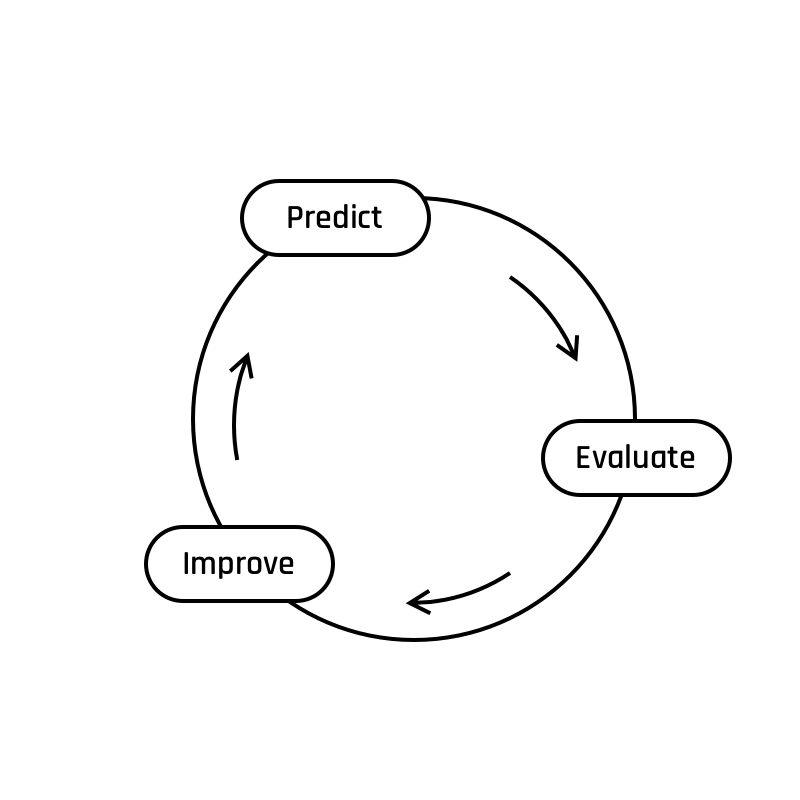
\includegraphics[scale=0.25]{assets/Default.png}
  \caption{cycle neutral}
\end{figure}

\section*{Predict}

\begin{figure}[h!]
  \centering
  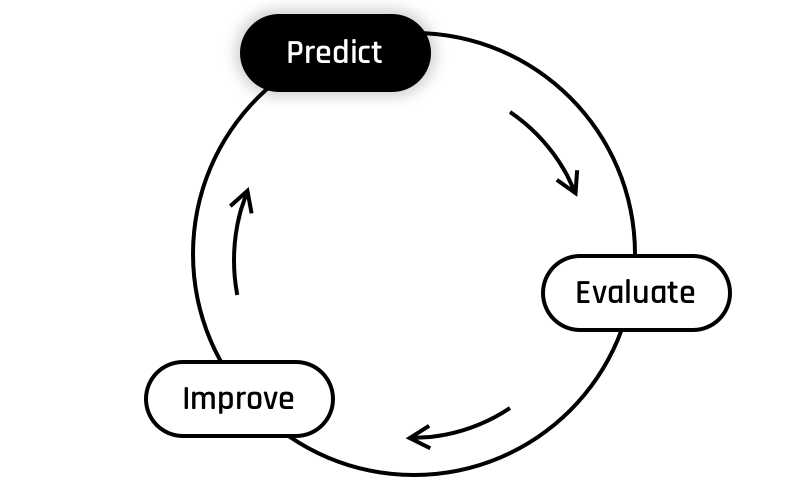
\includegraphics[scale=0.25]{assets/Predict.png}
  \caption{cycle predict}
\end{figure}

\subsection*{A very simple model}

We have some data. We want to model it.  
\begin{itemize}
    \item First we need to \textit{make an assumption}, or hypothesis, \textit{about the structure of the data and the relationship between the variables}.  
    \item Then we can \textit{apply that hypothesis to our data to make predictions}.
\end{itemize}

$$
hypothesis(data) = predictions
$$

\subsubsection*{Hypothesis}
Let's start with a very simple and intuitive \textbf{hypothesis} on how the price of a spaceship can be predicted based on the power of its engines.\\
We will consider that \textit{the more powerful the engines are, the more expensive the spaceship is}.\\
Furthermore, we will assume that the price increase is \textbf{proportional} to the power increase. In other words, we will look for a \textbf{linear relationship} between the two variables.

This means that we will formulate the price prediction with a \textbf{linear equation}, that you might be already familiar with:

$$
\hat{y} = ax + b
$$

We add the \texttt{\^} symbol over the $y$ to specify that $\hat{y}$ \textit{(pronounced y-hat)} is a \textbf{prediction} (or estimation) of the real value of $y$. The prediction is calculated with the \textbf{parameters} $a$ and $b$ and the input value $x$.

For example, if $a = 5$ and $b = 33$, then $\hat{y} = 5x + 33$.

But in Machine Learning, we don't like using the letters $a$ and $b$. Instead we will use the following notation:

$$
\hat{y} = \theta_0 + \theta_1 x
$$

So if $\theta_0 = 33$ and $\theta_1 = 5$, then $\hat{y} = 33+ 5x$.

To recap, this linear equation is our \textbf{hypothesis}. Then, all we will need to do is find the right values for our parameters $\theta_0$ and $\theta_1$ and we will get a fully-functional prediction \textbf{model}.


\subsubsection*{Predictions}
Now, how can we generate a set of predictions on an entire dataset? Let's consider a dataset containing $m$ data points (or space ships), called \textbf{examples}.

What we do is stack the $x$ and $\hat{y}$ values of all examples in vectors of length $m$. The relation between the elements in our vectors can then be represented with the following formula:

$$
\begin{matrix}
\hat{y}^{(i)} = \theta_0 + \theta_1 x^{(i)} & & \text{ for i = 1, ..., m}
\end{matrix}
$$  

Where:
\begin{itemize}
    \item $\hat{y}^{(i)}$ is the $i^{th}$ component of vector $y$
    \item $x^{(i)}$ is the $i^{th}$ component of vector $x$   
\end{itemize}

Which can be experessed as:

$$
\hat{y} = \begin{bmatrix}\theta_0 + \theta_1 \times x^{(1)} \\ \vdots \\  \theta_0 + \theta_1 \times x^{(m)}\ \end{bmatrix}
$$  

For example,

$$
\text{given } \theta = \begin{bmatrix}33 \\ 5 \end{bmatrix} \text{ and } x = \begin{bmatrix}1 \\ 3 \end{bmatrix} \text{: }
$$

$$
\hat{y} = h_{\theta}(x) = \begin{bmatrix} 33 +  5 \times 1 \\ 33 + 5 \times 3\end{bmatrix}  = \begin{bmatrix} 38 \\ 48 \end{bmatrix} 
$$

\newpage

\subsection*{More information}

\subsubsection*{Why the $\theta$ notation?}

You might have two questions at the moment:
\begin{itemize}
    \item \textbf{WTF is that weird  symbol?}
    This strange symbol, $\theta$, is called "theta".
    
    \item \textbf{Why use this notation instead of $a$ and $b$, like we're used to?}
    Despite its seeming more complicated at first, the theta notation is actually meant to simplify your equations later on. Why?
    $a$ and $b$ are good for a model with two parameters, but you will soon need to build more complex models that take into account more variables than just $x$.
    You could add more letters like this:  $\hat{y} = ax_1 + bx_2 + cx_3 + ... + yx_{25} + z$  
    But how do you go beyond 26 parameters? And how easily can you tell what parameter is associated with, let's say, $x_{19}$? That's why it becomes more handy to describe all your parameters using the theta notation and indices.
    With $\theta$, you just have to increment the number to name the parameter:
    $\hat{y} = \theta_0 + \theta_1 x_1 + \theta_2 x_2 + ... + \theta_{2468} x_{2468}$ ... Easy right?
\end{itemize}


\subsubsection*{Another common notation}

$$
\begin{matrix} & & \hat{y} & = & h_{\theta}(x)\end{matrix}
$$

Because $\hat{y}$ is calculated with our linear hypothesis using $\theta$ and $x$, it is sometimes written as $h_{\theta}(x)$.
The $h$ stands for \textit{hypothesis}, and can be read as \textit{"the result of our hypothesis h given x and theta"}.

Then if $x = 7$, we can calculate:
$\hat{y} = h_{\theta}(x) = 33 + 5 \times 7 = 68$
We can now say that according to our linear model, the \textbf{predicted value} of $y$ given ($x = 7$) is 68.

\newpage
\extitle{Simple Prediction}
\turnindir{ex02}
\exnumber{02}
\exfiles{prediction.py}
\exforbidden{any functions which performs prediction}
\makeheaderfilesforbidden

% ================================= %
\section*{Objective}
% --------------------------------- %
Understand and manipulate the notion of hypothesis in machine learning.

You must implement the following formula as a function:  
$$
\begin{matrix}
\hat{y}^{(i)} = \theta_0 + \theta_1 x^{(i)} & &\text{ for i = 1, ..., m}
\end{matrix}
$$  

Where:
\begin{itemize}
  \item $x$ is a vector of dimension $m$, the vector of examples/features (without the $y$ values),
  \item $\hat{y}$ is a vector of dimension m * 1, the vector of predicted values,
  \item $\theta$ is a vector of dimension 2 * 1, the vector of parameters,
  \item $y^{(i)}$ is the $i^{th}$ component of vector $y$,
  \item $x^{(i)}$ is the $i^{th}$ component of vector $x$.
\end{itemize}

% ================================= %
\section*{Instructions}
% --------------------------------- %
In the prediction.py file, write the following function as per the instructions given below:

\begin{minted}[bgcolor=darcula-back,formatcom=\color{lightgrey},fontsize=\scriptsize]{python}
def simple_predict(x, theta):
    """Computes the vector of prediction y_hat from two non-empty numpy.ndarray.
    Args:
      x: has to be an numpy.ndarray, a vector of dimension m * 1.
      theta: has to be an numpy.ndarray, a vector of dimension 2 * 1.
    Returns:
      y_hat as a numpy.ndarray, a vector of dimension m * 1.
      None if x or theta are empty numpy.ndarray.
      None if x or theta dimensions are not appropriate.
    Raises:
      This function should not raise any Exception.
    """
    ... Your code ...
\end{minted}

% ================================= %
\section*{Examples}
% --------------------------------- %
\begin{minted}[bgcolor=darcula-back,formatcom=\color{lightgrey},fontsize=\scriptsize]{python}
import numpy as np
x = np.arange(1,6)

# Example 1:
theta1 = np.array([5, 0])
simple_predict(x, theta1)
# Ouput:
array([5., 5., 5., 5., 5.])
# Do you understand why y_hat contains only 5's here?  


# Example 2:
theta2 = np.array([0, 1])
simple_predict(x, theta2)
# Output:
array([1., 2., 3., 4., 5.])
# Do you understand why y_hat == x here?  


# Example 3:
theta3 = np.array([5, 3])
simple_predict(x, theta3)
# Output:
array([ 8., 11., 14., 17., 20.])


# Example 4:
theta4 = np.array([-3, 1])
simple_predict(x, theta4)
# Output:
array([-2., -1.,  0.,  1.,  2.])  
\end{minted}


% ===========================(fin ex 02)         %
% ============================================== %

\newpage

% ============================================== %
% ===========================(start ex 03)       %
\chapter{Exercise 03}
%******************************************************************************%
%                                                                              %
%                                 Interlude                                    %
%                         for Machine Learning module                          %
%                                                                              %
%******************************************************************************%

% =============================== %
\section*{Interlude}
% =============================== %
\subsection*{Linear Algebra Strikes Again!}
% ******************************* %

You've become quite used to vectorization by now.
You may have already tried to vectorize the logistic loss function by yourself.
Let's look one last time at the former equation:

$$
J( \theta) = -\cfrac{1} {m} \lbrack \sum_{i = 1}^{m} y^{(i)}\log(\hat{y}^{(i)})) + (1 - y^{(i)})\log(1 - \hat{y}^{(i)})\rbrack
$$

% =============================== %
\subsection*{Vectorized Logistic Loss Function}
% ******************************* %
In the \textbf{vectorized version}, we remove the sum ($\sum$) because it is captured by the dot products:
$$
J( \theta) = -\cfrac{1} {m} \lbrack y \cdot \log(\hat{y}) + (\vec{1} - y) \cdot \log(\vec{1} - \hat{y})\rbrack
$$

Where:
\begin{itemize}
       \item $\vec{1}$ is a vector full of $1$'s with the same dimension of $y$ ($m$).
             $$
             \vec{1} = \begin{bmatrix}
                 1 \\
                 \vdots \\
                 1
             \end{bmatrix}
             $$
\end{itemize}


% =============================== %
\subsection*{Note: Operations Between Vectors and Scalars}
% ******************************* %
We use the $\vec{1}$ notation to be rigorous, because \textbf{addition (or subtraction) between a vector and a scalar is not defined}.
In other words, mathematically, you cannot write this: $1 - y$.
The only operation defined between a scalar and a vector is multiplication, remember?

% =============================== %
\subsubsection*{However...}
% ******************************* %
\texttt{NumPy} is a bit permissive on vectors and matrix operations...
The following instructions will get you the same results:

\begin{minted}[bgcolor=darcula-back,formatcom=\color{lightgrey},fontsize=\scriptsize]{python}
# Proper mathematical notation
y = np.array([[4], [7.16], [3.2], [9.37], [0.56]])
ones = np.ones(y.shape[0]).reshape((-1,1))
ones - y
# Output
array([[-3.  ],
       [-6.16],
       [-2.2 ],
       [-8.37],
       [ 0.44]])

# Incorrect mathematical notation
y = np.array([[4], [7.16], [3.2], [9.37], [0.56]])
1 - y
# Output
array([[-3.  ],
       [-6.16],
       [-2.2 ],
       [-8.37],
       [ 0.44]])
\end{minted}

Strange, isn't it?
It happens because of one of \texttt{NumPy}'s permissive operations called \textbf{Broadcasting}.
Broadcasting is a powerful feature whereby \texttt{NumPy} is able to figure out that you actually wanted to perform a subtraction on each element in the vector, so it does it for you automatically.
It's very handy to write concise lines of code, but it can insert very sneaky bugs if you aren't $100$\% confident in what you're doing.


Many of the bugs you will encounter while working on Machine Learning problems will come from \texttt{NumPy}'s permissiveness.
Such bugs generaly don't throw any errors, but mess up the content of your vectors and matrices and you'll spend an awful lot of time looking for why your model doesn't learn.
This is why we \textbf{strongly} suggest that you pay attention to your vector (and matrix) shapes and \textbf{stick as much as possible to the actual mathematical operations}.

For more information, you can watch \href{https://www.youtube.com/watch?v=V2QlTmh6P2Y&t=213s}{this video on dealing with Broadcasting}.

\newpage
\extitle{Add Intercept}
\turnindir{ex03}
\exnumber{03}
\exfiles{tools.py}
\exforbidden{None}
\makeheaderfilesforbidden

% ================================= %
\section*{Objective}
% --------------------------------- %
Understand and manipulate the notion of hypothesis in machine learning.
You must implement a function which adds an extra column of $1$'s on the left side of a given vector or matrix.

% ================================= %
\section*{Instructions}
% --------------------------------- %
In the tools.py file create the following function as per the instructions given below:

\begin{minted}[bgcolor=darcula-back,formatcom=\color{lightgrey},fontsize=\scriptsize]{python}
def add_intercept(x):
    """Adds a column of 1's to the non-empty numpy.array x.
    Args:
      x: has to be a numpy.array of dimension m * n.
    Returns:
      X, a numpy.array of dimension m * (n + 1).
      None if x is not a numpy.array.
      None if x is an empty numpy.array.
    Raises:
      This function should not raise any Exception.
    """
    ... Your code ...
\end{minted}

% ================================= %
\section*{Examples}
% --------------------------------- %

\begin{minted}[bgcolor=darcula-back,formatcom=\color{lightgrey},fontsize=\scriptsize]{python}
import numpy as np

# Example 1:
x = np.arange(1,6)
add_intercept(x)
# Output:
array([[1., 1.],
       [1., 2.],
       [1., 3.],
       [1., 4.],
       [1., 5.]])


# Example 2:
y = np.arange(1,10).reshape((3,3))
add_intercept(y)
# Output:
array([[1., 1., 2., 3.],
       [1., 4., 5., 6.],
       [1., 7., 8., 9.]])
\end{minted}


% ===========================(fin ex 03)         %
% ============================================== %

\newpage

% ============================================== %
% ===========================(start ex 04)       %
\chapter{Exercise 04}
\extitle{Prediction}
\turnindir{ex04}
\exnumber{04}
\exfiles{prediction.py}
\exforbidden{None}
\makeheaderfilesforbidden


% ================================= %
\section*{Objective}
% --------------------------------- %
Understand and manipulate the notion of hypothesis in machine learning.

You must implement the following formula as a function: 

$$
\begin{matrix}
\hat{y}^{(i)} = \theta_0 + \theta_1 x^{(i)} & &\text{ for i = 1, ..., m}
\end{matrix}
$$  

Where:
\begin{itemize}
  \item $\hat{y}^{(i)}$ is the $i^{th}$ component of vector $\hat{y}$
  \item $\hat{y}$ is a vector of dimension $m$, the vector of predicted values
  \item $\theta$ is a vector of dimension $2 \times 1$, the vector of parameters
  \item $x^{(i)}$ is the $i^{th}$ component of vector $x$  
  \item $x$ is a vector of dimension $m$, the vector of examples
\end{itemize}

But this time you have to do it with the linear algebra trick!

$$
\hat{y} = X' \cdot \theta = 
\begin{bmatrix} 
1 & x^{(1)} \\ 
\vdots & \vdots \\ 
1 & x^{(m)} 
\end{bmatrix} 
\cdot
\begin{bmatrix}
\theta_0 \\ 
\theta_1 
\end{bmatrix} 
 = \begin{bmatrix} 
\theta_0 + \theta_1x^{(1)} \\ 
\vdots \\ 
\theta_0 + \theta_1x^{(m)} 
\end{bmatrix} 
$$

\warn{
\begin{itemize}
  \item the argument $x$ is an $m$ vector
  \item $\theta$ is a $2 \times 1$ vector. 
\end{itemize}
}

You have to transform $x$ into $X'$ to fit the dimension of $\theta$!


% ================================= %
\section*{Instructions}
% --------------------------------- %
In the prediction.py file create the following function as per the instructions given below:

\begin{minted}[bgcolor=darcula-back,formatcom=\color{lightgrey},fontsize=\scriptsize]{python}
def predict_(x, theta):
    """Computes the vector of prediction y_hat from two non-empty numpy.array.
    Args:
      x: has to be an numpy.array, a vector of dimension m * 1.
      theta: has to be an numpy.array, a vector of dimension 2 * 1.
    Returns:
      y_hat as a numpy.array, a vector of dimension m * 1.
      None if x and/or theta are not numpy.array.
      None if x or theta are empty numpy.array.
      None if x or theta dimensions are not appropriate.
    Raises:
      This function should not raise any Exceptions.
    """
    ... Your code ...
\end{minted}

\section*{Examples}
\begin{minted}[bgcolor=darcula-back,formatcom=\color{lightgrey},fontsize=\scriptsize]{python}
import numpy as np
x = np.arange(1,6)

# Example 1:
theta1 = np.array([5, 0])
predict_(x, theta1)
# Ouput:
array([5., 5., 5., 5., 5.])
# Do you remember why y_hat contains only 5's here?

# Example 2:
theta2 = np.array([0, 1])
predict_(x, theta2)
# Output:
array([1., 2., 3., 4., 5.])
# Do you remember why y_hat == x here?

# Example 3:
theta3 = np.array([5, 3])
predict_(X, theta3)
# Output:
array([ 8., 11., 14., 17., 20.])


# Example 4:
theta4 = np.array([-3, 1])
predict_(x, theta4)
# Output:
array([-2., -1.,  0.,  1.,  2.])
\end{minted}

% ===========================(fin ex 04)         %
% ============================================== %

\newpage

% ============================================== %
% ===========================(start ex 05)       %
\chapter{Exercise 05}
\extitle{Let’s Make Nice Plots}
\turnindir{ex05}
\exnumber{05}
\exfiles{plot.py}
\exforbidden{None}
\makeheaderfilesforbidden

\info{
  For you information, the task we are performing here is called \textbf{regression}.
  It means that we are trying to predict a continuous numerical attribute for all examples (like a price, for instance).
  Later in the bootcamp, you will see that we can predict other things such as categories.
}

% ================================= %
\section*{Objective}
% --------------------------------- %
You must implement a function to plot the data and the prediction line (or regression line).  
You will plot the data points (with their x and y values), and the prediction line that represents your hypothesis ($h_{\theta}$).

\newpage

% ================================= %
\section*{Instructions}
% --------------------------------- %
In the plot.py file, create the following function as per the instructions given below:

\begin{minted}[bgcolor=darcula-back,formatcom=\color{lightgrey},fontsize=\scriptsize]{python}
def plot(x, y, theta):
    """Plot the data and prediction line from three non-empty numpy.array.
    Args:
      x: has to be an numpy.array, a vector of dimension m * 1.
      y: has to be an numpy.array, a vector of dimension m * 1.
      theta: has to be an numpy.array, a vector of dimension 2 * 1.
    Returns:
        Nothing.
    Raises:
      This function should not raise any Exceptions.
    """
    ... Your code ...
\end{minted}

% ================================= %
\section*{Examples}
% --------------------------------- %

\begin{minted}[bgcolor=darcula-back,formatcom=\color{lightgrey},fontsize=\scriptsize]{python}
import numpy as np
x = np.arange(1,6)
y = np.array([3.74013816, 3.61473236, 4.57655287, 4.66793434, 5.95585554])

# Example 1:
theta1 = np.array([[4.5],[-0.2]])
plot(x, y, theta1)
# Output:
\end{minted}

\begin{figure}[H]
  \centering
  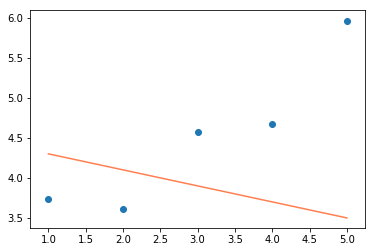
\includegraphics[scale=0.6]{assets/plot1.png}
\end{figure}

\newpage

\begin{minted}[bgcolor=darcula-back,formatcom=\color{lightgrey},fontsize=\scriptsize]{python}
# Example 2:
theta2 = np.array([[-1.5],[2]])
plot(x, y, theta2)
# Output:
\end{minted}

\begin{figure}[H]
  \centering
  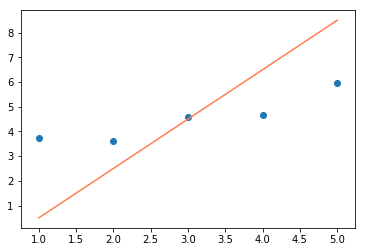
\includegraphics[scale=0.6]{assets/plot2.png}
  \caption{Example 2}
\end{figure}

\begin{minted}[bgcolor=darcula-back,formatcom=\color{lightgrey},fontsize=\scriptsize]{python}
# Example 3:
theta3 = np.array([[3],[0.3]])
plot(x, y, theta3)
# Output:
\end{minted}

\begin{figure}[H]
  \centering
  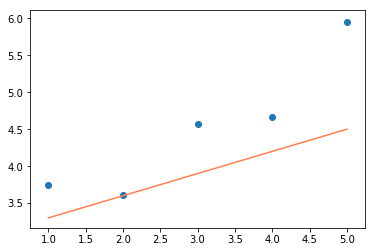
\includegraphics[scale=0.6]{assets/plot3.png}
  \caption{Example 3}
\end{figure}


% ===========================(fin ex 05)         %
% ============================================== %

\newpage

% ============================================== %
% ===========================(start ex 06)       %
\chapter{Exercise 06}
%******************************************************************************%
%                                                                              %
%                                 Interlude                                    %
%                         for Machine Learning module                          %
%                                                                              %
%******************************************************************************%

\section*{Interlude - Evaluate}

\begin{figure}[h!]
  \centering
  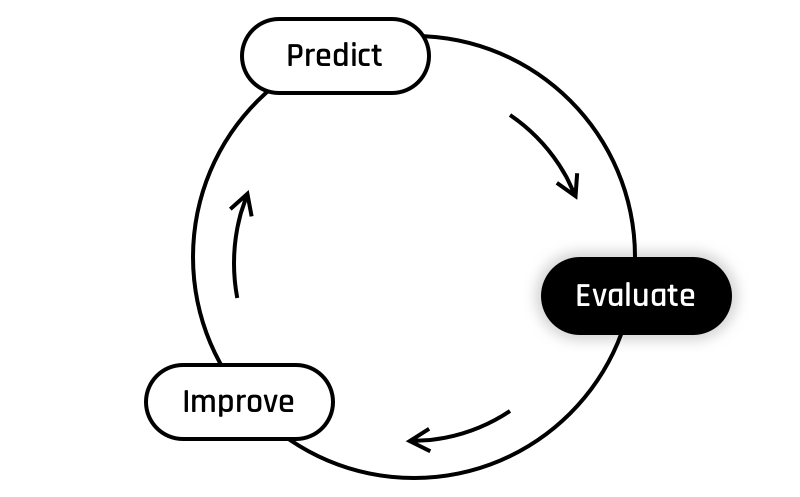
\includegraphics[scale=0.25]{assets/Evaluate.png}
  % \caption{cycle evaluate}
\end{figure}

\subsection*{Introducing the loss function}

How good is our model?  
It is hard to say just by simply looking at the plots!
We can clearly observe that certain regression lines seem to fit the data better than others, but it would be convenient to find a way to measure it. 

\begin{figure}[h!]
  \centering
  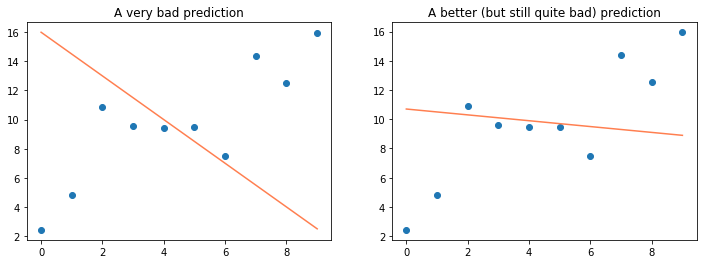
\includegraphics[scale=0.55]{assets/bad_prediction.png}
  \caption{bad prediction}
\end{figure}

To evaluate our model, we are going to use a \textbf{metric} called \textbf{the loss function} (sometimes called \textbf{cost function}).\\
\newline
The loss function tells us how bad our model is performing, how much it \textit{costs} us to use it, how much information we \textit{lose} when we use it.
If the model is good, we won't lose that much; if it's terrible instead, we will have a high loss!

The metric you choose will deeply impact the evaluation (and therefore also the training) of your model.

A frequent way to evaluate the performance of a regression model is to measure the distance between each predicted value ($\hat{y}^{(i)}$) and the real value it tries to predict (${y}^{(i)}$). The distances are then squared, and averaged to get one single metric, denoted $J$:

$$
J(\theta) = \frac{1}{2m}\sum_{i=1}^{m}(\hat{y}^{(i)} - y^{(i)})^2
$$

The smaller, the better! 

\begin{figure}[h!]
  \centering
  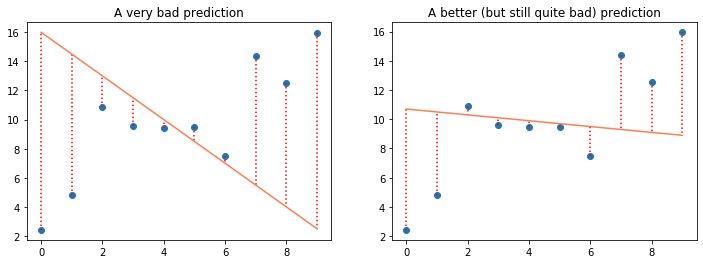
\includegraphics[scale=0.55]{assets/bad_pred_with_distance.png}
  \caption{bad prediction with distance}
\end{figure}

\newpage
\extitle{Loss function}
\turnindir{ex06}
\exnumber{06}
\exfiles{loss.py}
\exforbidden{None}
\makeheaderfilesforbidden


% ================================= %
\section*{Objective}
% --------------------------------- %
Understand and manipulate the notion of loss function in machine learning.

You must implement the following formula as a function (and another one very close to it):

$$
J(\theta) = \frac{1}{2m}\sum_{i=1}^{m}(\hat{y}^{(i)} - y^{(i)})^2
$$

Where:
\begin{itemize}
  \item $\hat{y}$ is a vector of dimension $m$, the vector of predicted values
  \item $y$ is a vector of dimension $m\times 1$, the vector of expected values
  \item $\hat{y}^{(i)}$ is the ith component of vector $\hat{y}$,
  \item $y^{(i)}$ is the ith component of vector $y$,
\end{itemize}

\newpage

% ================================= %
\section*{Instructions}
% --------------------------------- %
The implementation of the loss function has been split in two functions:
\begin{itemize}
  \item \texttt{loss\_elem\_()}, which computes the squared distances for all examples ($\hat{y}^{(i)} - y^{(i)})^2$),
  \item \texttt{loss\_()}, which averages the squared distances of all examples (the $J_(\theta)$ above).
\end{itemize}

In the loss.py file create the following functions as per the instructions given below:
\par
\begin{minted}[bgcolor=darcula-back,formatcom=\color{lightgrey},fontsize=\scriptsize]{python}
def loss_elem_(y, y_hat):
	"""
	Description:
		Calculates all the elements (y_pred - y)^2 of the loss function.
	Args:
      y: has to be an numpy.array, a vector.
      y_hat: has to be an numpy.array, a vector.
	Returns:
		J_elem: numpy.array, a vector of dimension (number of the training examples,1).
		None if there is a dimension matching problem between X, Y or theta.
		None if any argument is not of the expected type.
	Raises:
		This function should not raise any Exception.
	"""
	... your code here ...

def loss_(y, y_hat):
	"""
	Description:
		Calculates the value of loss function.
	Args:
      y: has to be an numpy.array, a vector.
      y_hat: has to be an numpy.array, a vector.
	Returns:
		J_value : has to be a float.
		None if there is a dimension matching problem between X, Y or theta.
		None if any argument is not of the expected type.
	Raises:
		This function should not raise any Exception.
	"""
	... your code here ...
\end{minted}

% ================================= %
\section*{Examples}
% --------------------------------- %
\begin{minted}[bgcolor=darcula-back,formatcom=\color{lightgrey},fontsize=\scriptsize]{python}
import numpy as np

x1 = np.array([[0.], [1.], [2.], [3.], [4.]])
theta1 = np.array([[2.], [4.]])
y_hat1 = predict_(x1, theta1)
y1 = np.array([[2.], [7.], [12.], [17.], [22.]])

# Example 1:
loss_elem_(y1, y_hat1)

# Output:
array([[0.], [1], [4], [9], [16]])

# Example 2:
loss_(y1, y_hat1)

# Output:
3.0

x2 = np.array([[0.2, 2., 20.], [0.4, 4., 40.], [0.6, 6., 60.], [0.8, 8., 80.]])
theta2 = np.array([[0.05], [1.], [1.], [1.]])
y_hat2 = predict_(x2, theta2)
y2 = np.array([[19.], [42.], [67.], [93.]])

# Example 3:
loss_elem_(y2, y_hat2)

# Output:
array([[10.5625], [ 6.0025], [ 0.1225], [17.2225]])

# Example 4:
loss_(y2, y_hat2)

# Output:
4.238750000000004

x3 = np.array([0, 15, -9, 7, 12, 3, -21])
theta3 = np.array([[0.], [1.]])
y_hat3 = predict_(x3, theta3)
y3 = np.array([2, 14, -13, 5, 12, 4, -19])

# Example 5:
loss_(y3, y_hat3)

# Output:
2.142857142857143

# Example 6:
loss_(y3, y3)

# Output:
0.0
\end{minted}

\info{
  This loss function is very close to the one called \textbf{"Mean Squared Error"}, which is frequently mentioned in Machine Learning resources.
  The difference is in the denominator as you can see in the formula of the $MSE = \frac{1}{m}\sum_{i=1}^{m}(\hat{y}^{(i)} - y^{(i)})^2$.
  
  Except the division by $2m$ instead of $m$, these functions are rigourously identical: $J(\theta) = \frac{MSE}{2}$.  
  
  MSE is called like that because it represents the mean of the errors (i.e.: the differences between the predicted values and the true values), squared.
  
  You might wonder why we choose to divide by two instead of simply using the MSE?  
  \textbf{(It's a good question, by the way.)}
  \begin{itemize}
    \item First, it does not change the overall model evaluation: if all performance measures are divided by two, we can still compare different models and their performance ranking will remain the same.
    \item Second, it will be convenient when we will calculate the gradient tomorow. Be patient, and trust us ;)
  \end{itemize}
  }
  
  % ===========================(fin ex 06)         %
  % ============================================== %
  
  \newpage
  
  % ============================================== %
  % ===========================(start ex 07)       %
  \chapter{Exercise 07}
  \extitle{Vectorized loss function}
  \turnindir{ex07}
  \exnumber{07}
  \exfiles{vec\_loss.py}
  \exforbidden{None}
  \makeheaderfilesforbidden
  
% ================================= %
\section*{Objective}
% --------------------------------- %
Understand and manipulate the notion of loss function in machine learning.
  
You must implement the following formula as a function:  
$$
\begin{matrix}
  J(\theta) &  = & \frac{1}{2m}(\hat{y} - y) \cdot(\hat{y}- y)
\end{matrix}
$$

Where:
\begin{itemize}
  \item $\hat{y}$ is a vector of dimension $m$, the vector of predicted values,
  \item $y$ is a vector of dimension $m$, the vector of expected values.
\end{itemize}

\newpage

% ================================= %
\section*{Instructions}
% --------------------------------- %
In the \texttt{vec\_loss.py} file, create the following function as per the instructions given below:

\begin{minted}[bgcolor=darcula-back,formatcom=\color{lightgrey},fontsize=\scriptsize]{python}
def loss_(y, y_hat):
    """Computes the half mean squared error of two non-empty numpy.array, without any for loop.
    The two arrays must have the same dimensions.
    Args:
      y: has to be an numpy.array, a vector.
      y_hat: has to be an numpy.array, a vector.
    Returns:
      The half mean squared error of the two vectors as a float.
      None if y or y_hat are empty numpy.array.
      None if y and y_hat does not share the same dimensions.
    Raises:
      This function should not raise any Exceptions.
    """
    ... Your code ...
\end{minted}


% ================================= %
\section*{Examples}
% --------------------------------- %
\begin{minted}[bgcolor=darcula-back,formatcom=\color{lightgrey},fontsize=\scriptsize]{python}
import numpy as np
X = np.array([0, 15, -9, 7, 12, 3, -21])
Y = np.array([2, 14, -13, 5, 12, 4, -19])

# Example 1:
loss_(X, Y)
# Output:
2.142857142857143

# Example 2:
loss_(X, X)
# Output:
0.0
\end{minted}

% ===========================(fin ex 07)         %
% ============================================== %

\newpage

% ============================================== %
% ===========================(start ex 08)       %
\chapter{Exercise 08}
%******************************************************************************%
%                                                                              %
%                                 Interlude                                    %
%                         for Machine Learning module                          %
%                                                                              %
%******************************************************************************%

\section*{Interlude - Fifty Shades of Linear Algebra}

In the last exercise, we implemented the loss function in two subfunctions.
It worked, but it's not very pretty.
What if we could do it all in one step, with linear algebra?   

As we did with the hypothesis, we can use a vectorized equation to improve the calculations of the loss function.

So now let's look at how squaring and averaging can be performed (more or less) in a single matrix multiplication!

$$
J(\theta) = \frac{1}{2m}\sum_{i=1}^{m}(\hat{y}^{(i)} - y^{(i)})^2
$$
$$
J(\theta) = \frac{1}{2m}\sum_{i=1}^{m}[(\hat{y}^{(i)} - y^{(i)}) (\hat{y}^{(i)} - y^{(i)})]
$$

Now, if we apply the definition of the dot product:

$$
J(\theta) = \frac{1}{2m}(\hat{y} - y) \cdot(\hat{y}- y)
$$
\newpage
\extitle{Lets Make Nice Plots Again}
\turnindir{ex08}
\exnumber{08}
\exfiles{plot.py}
\exforbidden{None}
\makeheaderfilesforbidden


% ================================= %
\section*{Objective}
% --------------------------------- %
You must implement a function which plots the data, the prediction line, and the loss.  
You will plot the $x$ and $y$ coordinates of all data points as well as the prediction line generated by your theta parameters.
Your function must also display the overall loss ($J$) in the title, and draw small lines marking the distance between each data point and its predicted value.

% ================================= %
\section*{Instructions}
% --------------------------------- %
In the plot.py file create the following function as per the instructions given below:
\begin{minted}[bgcolor=darcula-back,formatcom=\color{lightgrey},fontsize=\scriptsize]{python}
def plot_with_loss(x, y, theta):
"""Plot the data and prediction line from three non-empty numpy.ndarray.
    Args:
      x: has to be an numpy.ndarray, a vector of dimension m * 1.
      y: has to be an numpy.ndarray, a vector of dimension m * 1.
      theta: has to be an numpy.ndarray, a vector of dimension 2 * 1.
    Returns:
        Nothing.
    Raises:
      This function should not raise any Exception.
    """
    ... Your code ...
\end{minted}

\newpage

% ================================= %
\section*{Examples}
% --------------------------------- %
\begin{minted}[bgcolor=darcula-back,formatcom=\color{lightgrey},fontsize=\scriptsize]{python}
import numpy as np
x = np.arange(1,6)
y = np.array([11.52434424, 10.62589482, 13.14755699, 18.60682298, 14.14329568])

# Example 1:
theta1= np.array([18,-1])
plot_with_loss(x, y, theta1)
# Output:
\end{minted}

\begin{figure}[H]
  \centering
  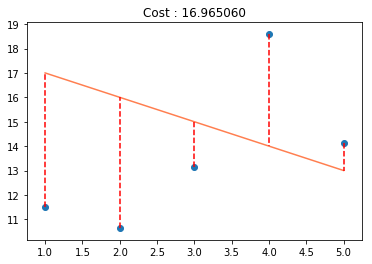
\includegraphics[scale=0.65]{assets/plotcost1.png}
  \caption{Example 1}
\end{figure}

\begin{minted}[bgcolor=darcula-back,formatcom=\color{lightgrey},fontsize=\scriptsize]{python}
# Example 2:
theta2 = np.array([14, 0])
plot_with_loss(x, y, theta2)
# Output:
\end{minted}

\begin{figure}[H]
  \centering
  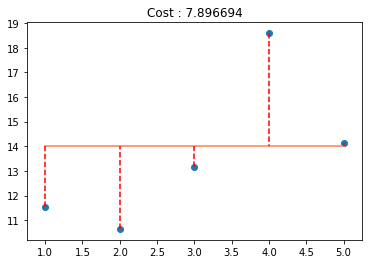
\includegraphics[scale=0.65]{assets/plotcost2.png}
  \caption{Example 2}
\end{figure}

\newpage

\begin{minted}[bgcolor=darcula-back,formatcom=\color{lightgrey},fontsize=\scriptsize]{python}
# Example 3:
theta3 = np.array([12, 0.8])
plot_with_loss(x, y, theta3)
# Output:
\end{minted}

\begin{figure}[H]
  \centering
  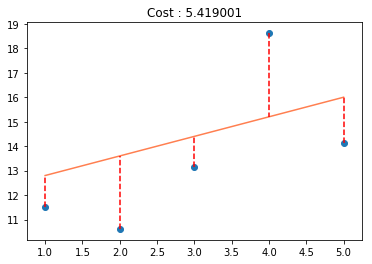
\includegraphics[scale=0.65]{assets/plotcost3.png}
  \caption{Example 3}
\end{figure}

% ===========================(fin ex 08)         %
% ============================================== %

\newpage

% ============================================== %
% ===========================(start ex 09)       %
\chapter{Exercise 09}
\extitle{Other loss functions}
\turnindir{ex09}
\exnumber{09}
\exfiles{other\_losses.py}
\exforbidden{None}
\makeheaderfilesforbidden

Deepen the notion of loss function in machine learning.

You certainly had a lot of fun implementing your loss function.
Remember we told you it was \textbf{one among many possible ways of measuring the loss}.
Now, you will get to implement other metrics.  You already know about one of them: \textbf{MSE}.  
There are several more which are quite common: \textbf{RMSE}, \textbf{MAE} and \textbf{R2score}.

\newpage

% ================================= %
\section*{Objective}
% --------------------------------- %
You must implement the following formulas as functions:

$$
MSE(y, \hat{y}) = \frac{1}{m}\sum_{i=1}^{m}(\hat{y}^{(i)} - y^{(i)})^2
$$

$$
RMSE(y, \hat{y}) = \sqrt{\frac{1}{m}\sum_{i=1}^{m}(\hat{y}^{(i)} - y^{(i)})^2}
$$

$$
MAE(y, \hat{y}) = \frac{1}{m}\sum_{i=1}^{m}|{\hat{y}^{(i)} - y^{(i)}}|
$$

$$
R^2(y, \hat{y}) = 1 - \frac{\sum_{i=1}^{m}(\hat{y}^{(i)} - y^{(i)})^2}{\sum_{i=1}^{m}({y}^{(i)} - \bar{y})^2}
$$

Where:
\begin{itemize}
  \item $y$ is a vector of dimension $m$,
  \item $\hat{y}$ is a vector of dimension $m$,
  \item $y^{(i)}$ is the $i^{th}$ component of vector $y$,
  \item $\hat{y}^{(i)}$ is the $i^{th}$ component of $\hat{y}$,
  \item $\bar{y}$ is the mean of the $y$ vector
\end{itemize}

\newpage

% ================================= %
\section*{Instructions}
% --------------------------------- %
In the \texttt{other\_losses.py} file, create the following functions: MSE, RMSE, MAE, R2score, as per the instructions given below:

\begin{minted}[bgcolor=darcula-back,formatcom=\color{lightgrey},fontsize=\scriptsize]{python}
def mse_(y, y_hat):
	"""
	Description:
		Calculate the MSE between the predicted output and the real output.
	Args:
        y: has to be a numpy.array, a vector of dimension m * 1.
        y_hat: has to be a numpy.array, a vector of dimension m * 1.		
	Returns:
		mse: has to be a float.
		None if there is a matching dimension problem.
	Raises:
		This function should not raise any Exceptions.
	"""
		... your code here ...
\end{minted}
\begin{minted}[bgcolor=darcula-back,formatcom=\color{lightgrey},fontsize=\scriptsize]{python}
def rmse_(y, y_hat):
	"""
	Description:
		Calculate the RMSE between the predicted output and the real output.
	Args:
	        y: has to be a numpy.array, a vector of dimension m * 1.
        y_hat: has to be a numpy.array, a vector of dimension m * 1.		
	Returns:
		rmse: has to be a float.
		None if there is a matching dimension problem.
	Raises:
		This function should not raise any Exceptions.
	"""
		... your code here ...
\end{minted}
\begin{minted}[bgcolor=darcula-back,formatcom=\color{lightgrey},fontsize=\scriptsize]{python}
def mae_(y, y_hat):
	"""
	Description:
		Calculate the MAE between the predicted output and the real output.
	Args:
        y: has to be a numpy.array, a vector of dimension m * 1.
        y_hat: has to be a numpy.array, a vector of dimension m * 1.		
	Returns:
		mae: has to be a float.
		None if there is a matching dimension problem.
	Raises:
		This function should not raise any Exceptions.
	"""
		... your code here ...
\end{minted}
\begin{minted}[bgcolor=darcula-back,formatcom=\color{lightgrey},fontsize=\scriptsize]{python}
def r2score_(y, y_hat):
	"""
	Description:
		Calculate the R2score between the predicted output and the output.
	Args:
        y: has to be a numpy.array, a vector of dimension m * 1.
        y_hat: has to be a numpy.array, a vector of dimension m * 1.		
	Returns:
		r2score: has to be a float.
		None if there is a matching dimension problem.
	Raises:
		This function should not raise any Exceptions.
	"""
		... your code here ...
\end{minted}

\hint{
  You might consider implementing four more methods, similar to what you did for the loss function in exercise 07:
\begin{itemize}
  \item \texttt{mse\_elem()},
  \item \texttt{rmse\_elem()},
  \item \texttt{mae\_elem()},
  \item \texttt{r2score\_elem()}.
\end{itemize}
}

% ================================= %
\section*{Examples}
% --------------------------------- %
\begin{minted}[bgcolor=darcula-back,formatcom=\color{lightgrey},fontsize=\scriptsize]{python}
import numpy as np
from sklearn.metrics import mean_squared_error, mean_absolute_error, r2_score
from math import sqrt

# Example 1:
x = np.array([0, 15, -9, 7, 12, 3, -21])
y = np.array([2, 14, -13, 5, 12, 4, -19])

# Mean squared error
## your implementation
mse_(x,y)
## Output:
4.285714285714286
## sklearn implementation
mean_squared_error(x,y)
## Output:
4.285714285714286

# Root mean squared error
## your implementation
rmse_(x,y)
## Output:
2.0701966780270626
## sklearn implementation not available: take the square root of MSE
sqrt(mean_squared_error(x,y))
## Output:
2.0701966780270626

# Mean absolute error
## your implementation
mae_(x,y)
# Output:
1.7142857142857142
## sklearn implementation
mean_absolute_error(x,y)
# Output:
1.7142857142857142

# R2-score
## your implementation
r2score_(x,y)
## Output:
0.9681721733858745
## sklearn implementation
r2_score(x,y)
## Output:
0.9681721733858745
\end{minted}

% ===========================(fin ex 09)         %
% ============================================== %

\newpage

% ============================================== %
% ===========================(start ex 10)       %
\chapter{Conclusion - What you have learned}

The excercises serie is finished, well done!
Based on all the knowledges tackled today, you should be able to discuss and answer the following questions:
\begin{enumerate}
  \item Why do we concatenate a column of ones to the left of the $x$ vector when we use the linear algebra trick?   
  
  \item Why does the loss function square the distances between the data points and their predicted values?
  
  \item What does the loss function's output represent?
  
  \item Toward which value do we want the loss function to tend? What would that mean? 
  
  \item Do you understand why are matrix multiplications are not commutative?
\end{enumerate}

These questions constitute an opportunity as peer community to explain for those you have not encountered these questions
or to exchange and developped your comprehension with peers who have think about those ones.

% ===========================(fin ex 10)         %
% ============================================== %

\newpage

% ================================= %
\section*{Contact}
% --------------------------------- %
You can contact 42AI association by email: contact@42ai.fr\\
You can join the association on \href{https://join.slack.com/t/42-ai/shared_invite/zt-ebccw5r7-YPkDM6xOiYRPjqJXkrKgcA}{42AI slack}
and/or posutale to \href{https://forms.gle/VAFuREWaLmaqZw2D8}{one of the association teams}.

% ================================= %
\section*{Acknowledgements}
% --------------------------------- %
The modules Python \& ML is the result of a collective work, we would like to thanks:
\begin{itemize}
  \item Maxime Choulika (cmaxime),
  \item Pierre Peigné (ppeigne),
  \item Matthieu David (mdavid).
\end{itemize}
who supervised the creation, the enhancement and this present transcription.

\begin{itemize}
  \item Amric Trudel (amric@42ai.fr)
  \item Benjamin Carlier (bcarlier@student.42.fr)
  \item Pablo Clement (pclement@student.42.fr)
\end{itemize}
for your investment for the creation and development of these modules.

\begin{itemize}
  \item Richard Blanc (riblanc@student.42.fr)
  \item Solveig Gaydon Ohl (sgaydon-@student.42.fr)
  \item Quentin Feuillade Montixi (qfeuilla@student.42.fr)
\end{itemize}
who betatest the first version of the modules of Machine Learning.
\vfill
\doclicenseThis
\end{document}
